\documentclass[conference]{IEEEtran}

\usepackage{amsmath}
\usepackage{amssymb}
\usepackage{array}
\usepackage{booktabs}
\usepackage{cite}
\usepackage{graphicx}
\usepackage{url}
\usepackage{xcolor}
\usepackage[hidelinks]{hyperref}

\newcommand{\placeholder}[1]{\textcolor{red}{[TODO: #1]}}
\newcommand{\vehicles}{\mathcal{X}}
\newcommand{\zones}{\mathcal{Z}}
\newcommand{\trajectories}{\mathcal{T}}

\title{Priority-Aware Constrained Job-Shop Scheduling for Autonomous Intersection Management}

\author{
\IEEEauthorblockN{[Author Name]}
\IEEEauthorblockA{[Institution]\\
Email: [email address]}
}

\begin{document}

\maketitle

\begin{abstract}
Autonomous intersection management (AIM) can replace fixed signal phases with a scheduling mechanism that coordinates connected and automated vehicles through shared conflict areas. A recent line of work models an intersection as a graph of conflict zones and transforms the resulting scheduling problem into a constrained job-shop scheduling problem (JSSP), enabling reinforcement-learning-based dispatching policies. This paper develops a priority-aware extension of that formulation for heterogeneous vehicles. Each vehicle is represented as a job with a release time, a predicted trajectory through conflict zones, class-dependent traversal properties, and a priority weight. The objective is to minimize weighted delay while preserving safety constraints, same-lane order, blocking feasibility, and deadlock avoidance. The proposed framework is designed for online receding-horizon operation, where arrival times and conflict-zone occupation times are predicted from vehicle states and the schedule is repeatedly updated as new vehicles enter the control region. The paper presents the mathematical formulation, a safety-aware learning and heuristic scheduling framework, and an evaluation design for comparing first-come-first-served, greedy, priority-greedy, optimization-based, and reinforcement-learning policies. This draft intentionally reports no experimental performance claims; it defines the formulation and validation plan for future implementation.
\end{abstract}

\begin{IEEEkeywords}
autonomous intersection management, connected and automated vehicles, job-shop scheduling, priority-aware scheduling, reinforcement learning, receding horizon control
\end{IEEEkeywords}

\section{Introduction}

Intersections are among the most important bottlenecks in urban road networks. Conventional signal control allocates right-of-way by phases, but the fixed or semi-fixed structure of signal phases can leave unused capacity when traffic is sparse and can impose unnecessary stops when vehicles could otherwise coordinate safely. Connected and automated vehicles (CAVs) change the intersection-control problem because vehicles can share position, speed, route, and intention information with a roadside controller or with each other. In a fully connected and automated setting, the intersection can be managed as a space-time resource allocation problem rather than as a fixed signal cycle.

Autonomous intersection management (AIM) was introduced as a reservation-based multiagent control problem in which vehicles request access to space-time regions of an intersection \cite{dresner2008multiagent}. Later work developed graph-based models that divide an intersection into conflict zones and verify collision-free and deadlock-free passing orders \cite{lin2019graph}. The connection to job-shop scheduling is natural: vehicles are jobs, conflict zones are machines or resources, and the traversal of a conflict zone is an operation. Huang et al. recently used this mapping to transform graph-based AIM into a constrained job-shop scheduling problem (JSSP) and trained a centralized intersection manager with proximal policy optimization (PPO) \cite{huang2023reinforcement}.

This paper develops a formulation-level extension of that direction. The main idea is that real traffic is heterogeneous. A passenger car, a bus, a truck, and an emergency vehicle should not necessarily be treated as identical jobs with identical delay costs. Buses may represent larger person-delay, trucks may require longer conflict-zone occupation and safety headway, and emergency vehicles may require hard or near-hard priority. At the same time, priority cannot relax physical safety: no vehicle class may violate conflict-zone capacity, trajectory order, same-lane order, blocking feasibility, or deadlock constraints.

The proposed contribution is a priority-aware constrained JSSP formulation for single-intersection AIM. Each vehicle is represented by an arrival or release time, a predicted trajectory through conflict zones, a class label, physical traversal parameters, and a priority weight. The scheduling objective minimizes weighted delay with an optional fairness term. The framework is designed for online receding-horizon execution, where the controller repeatedly predicts near-future vehicle arrivals, constructs a finite constrained-JSSP instance, schedules feasible operations, executes only near-term decisions, and re-plans as the traffic stream changes.

The paper makes the following formulation contributions:
\begin{itemize}
    \item It defines a priority-aware constrained-JSSP model for heterogeneous CAV intersection scheduling.
    \item It separates priority from safety: priority affects the objective or emergency constraints, while safety is enforced by resource, ordering, blocking, and deadlock constraints.
    \item It gives a receding-horizon scheduling architecture that can use kinematic or learned prediction of arrival and conflict-zone occupation times.
    \item It specifies non-learning and learning-based baselines for a future implementation, including FCFS, greedy, priority-greedy, deadlock-aware greedy, small-instance optimization, and PPO/GNN dispatching.
\end{itemize}

Fig.~\ref{fig:framework} summarizes the intended framework. The figure is included from the existing repository material and should be replaced by a publication-ready diagram before submission.

\begin{figure}[t]
    \centering
    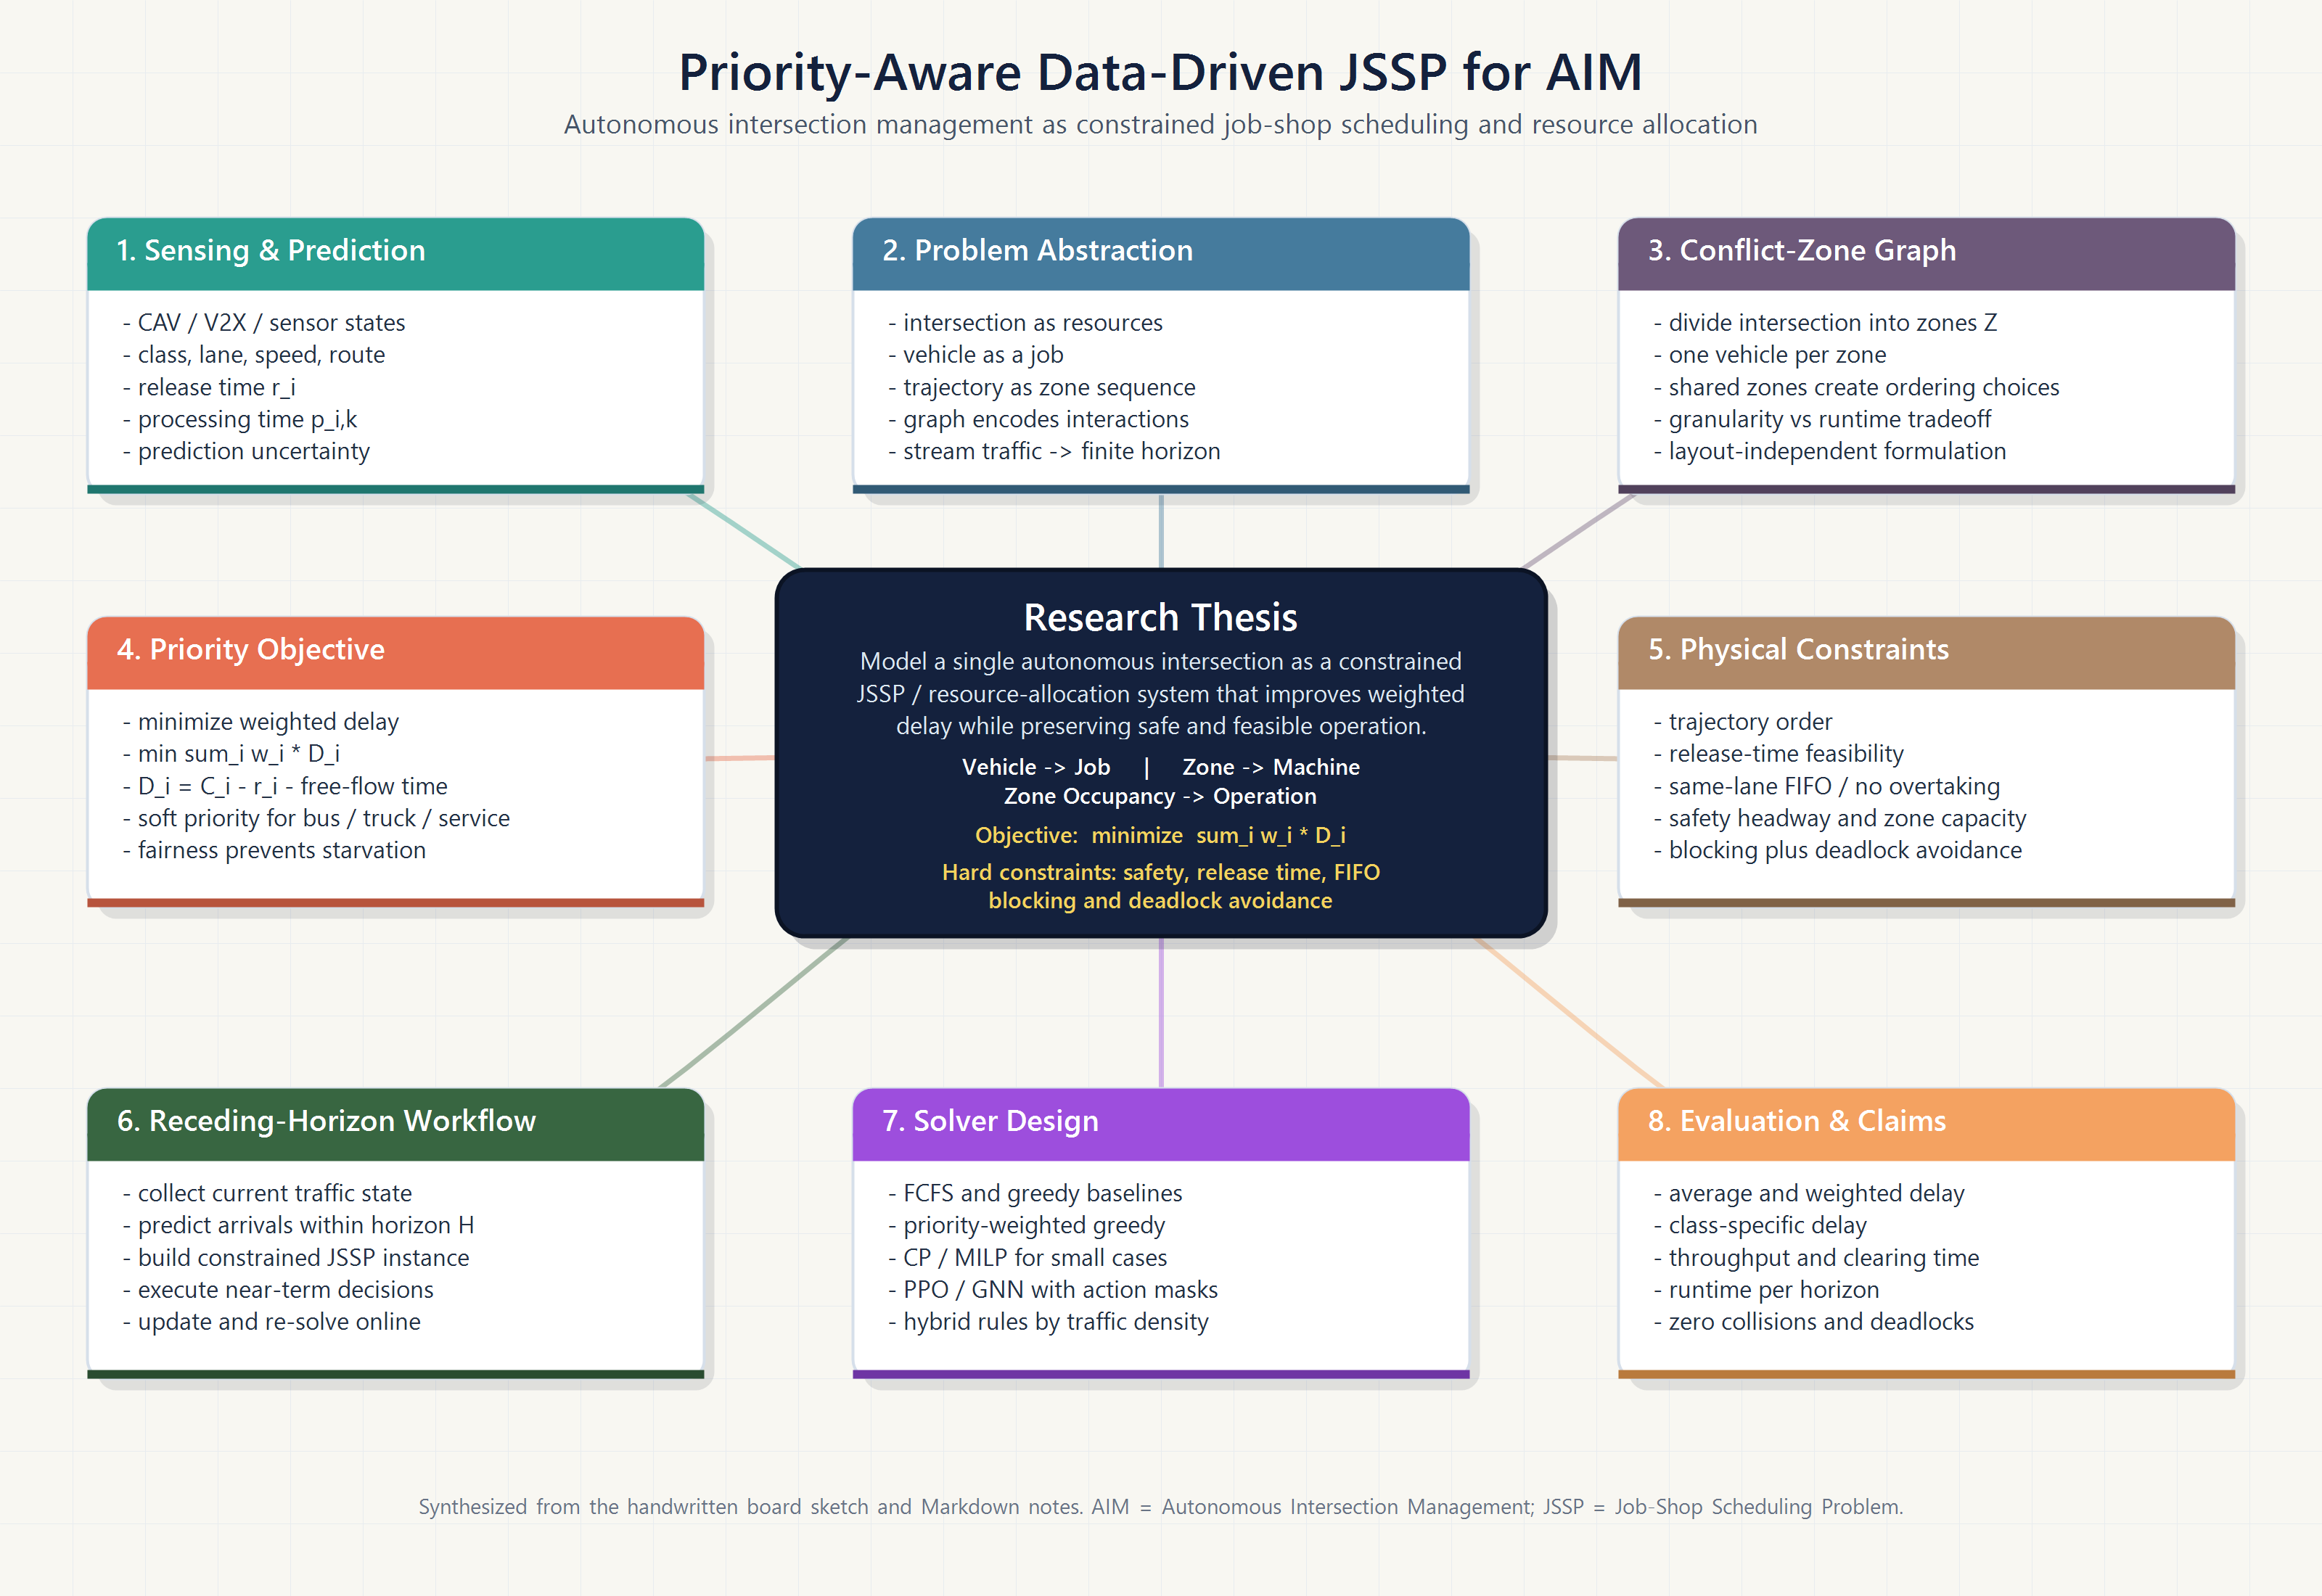
\includegraphics[width=\linewidth]{../../Pic/PriorityAwareJSSPAIMMindMap.png}
    \caption{Conceptual framework for priority-aware data-driven JSSP-based autonomous intersection management.}
    \label{fig:framework}
\end{figure}


\section{Related Work}

\subsection{Reservation-Based Autonomous Intersection Management}

Reservation-based AIM treats the intersection as a shared space-time resource. Dresner and Stone proposed a multiagent reservation protocol in which autonomous vehicles request intersection reservations and the intersection manager accepts or rejects those requests \cite{dresner2008multiagent}. That work established the central idea that signal-free intersections can coordinate autonomous vehicles more flexibly than traditional lights or stop signs, and it also considered mixed traffic and emergency-vehicle priority. Surveys by Chen and Englund \cite{chen2016cooperative}, Rios-Torres and Malikopoulos \cite{riosTorres2017survey}, and Khayatian et al. \cite{khayatian2020survey} organize later CAV intersection-management methods by communication architecture, safety guarantees, optimization method, and deployment challenges.

The present work follows the resource-allocation view of AIM but replaces simple request-order logic with a priority-aware scheduling formulation. This is important because first-come-first-served (FCFS) policies can be reasonable under low traffic density, yet may not exploit the full scheduling flexibility available when many vehicles compete for multiple conflict zones.

\subsection{Graph-Based Conflict-Zone Scheduling}

Graph-based AIM partitions the intersection into conflict zones and represents timing relationships between vehicle-zone pairs. Lin et al. introduced a graph-based model with formal deadlock-freeness analysis and a centralized cycle-removal scheduling algorithm \cite{lin2019graph}. Huang et al. later transformed this graph-based scheduling model into a constrained JSSP and trained a PPO policy for dispatching \cite{huang2023reinforcement}. Their formulation explicitly accounts for traffic-specific constraints, including blocking, deadlock, and arrival-time constraints. Ahn and Del Vecchio also used job-shop scheduling to verify intersection collision avoidance, showing that the scheduling abstraction is useful beyond purely manufacturing settings \cite{ahn2016semi}.

This paper keeps the graph/JSSP safety structure but adds heterogeneous priority and weighted delay. The resulting formulation is not a standard JSSP: it includes release times, physical vehicle-ordering constraints, traffic blocking, and deadlock prevention.

\subsection{Optimization-Based Scheduling and Rolling Horizon}

Mixed-integer optimization has been used to assign vehicle access times or reservations at autonomous intersections. Levin and Rey formulated intersection control with conflict points and proposed a rolling-horizon method for larger traffic streams \cite{levin2017conflict}. Fayazi and Vahidi proposed a mixed-integer linear programming (MILP) method for assigning optimal intersection access times to autonomous vehicles \cite{fayazi2018mixed}. Such exact formulations are valuable for small-instance validation, but their computational complexity can limit real-time deployment when many vehicles and conflict points are present.

Heterogeneous traffic has also been studied in scheduling formulations. Soleimaniamiri and Li considered heterogeneous vehicle headways and values of time at a general conflict area \cite{soleimaniamiri2019scheduling}. This supports the premise that vehicle classes should influence both physical constraints and scheduling objectives. Recent priority-based search methods also provide strong non-RL alternatives for intersection coordination, especially when the problem is viewed through multi-agent path finding \cite{li2023prioritysearch}.

\subsection{Reinforcement Learning for AIM and JSSP}

Reinforcement learning has been explored for centralized and decentralized AIM. Guan et al. used PPO for centralized CAV coordination at a signal-free intersection \cite{guan2020centralized}. Wu et al. proposed DCL-AIM, a decentralized coordination-learning method that decomposes state information to handle the dimensionality of multi-agent intersection control \cite{wu2019dcl}. Huang et al. applied RL specifically to graph-based AIM after transforming it into a constrained JSSP \cite{huang2023reinforcement}.

The JSSP literature also supports graph-based learning policies. Zhang et al. learned dispatching rules for JSSP using deep reinforcement learning \cite{zhang2020learning}. Their state is an evolving disjunctive graph with operation-level features such as a scheduled indicator and a completion-time lower bound; the action is to select one eligible operation; the transition schedules that operation at the earliest feasible machine slot and orients the corresponding disjunctive arcs; and the reward is tied to improvement in a makespan lower-bound objective. Park et al. similarly formulated JSSP scheduling with graph neural networks and PPO-style policy learning \cite{park2021learning}.

Huang et al. adapt this dispatching view to graph-based AIM by replacing generic jobs and machines with vehicles and conflict zones, and by adding traffic-specific feasibility filters for precedence, blocking, deadlock, and arrival time \cite{huang2023reinforcement}. Their reward is based on the extra vehicle delay introduced by a selected operation, and their grouping strategy clusters vehicle streams by arrival time so a policy trained on smaller groups can be applied online. These works motivate a graph encoder for vehicle-zone operations, conflict-zone resources, and precedence constraints. In the proposed AIM formulation, however, RL is not the source of safety. Safety must be enforced by feasibility masks, resource constraints, and verification checks, while the learned policy proposes efficient feasible dispatching actions.

\begin{table*}[t]
\centering
\caption{Relationship between generic JSSP-RL, JSSP-RL for AIM, and the proposed priority-aware formulation}
\label{tab:zhang-huang-proposed}
\scriptsize
\setlength{\tabcolsep}{3pt}
\begin{tabular}{p{0.16\textwidth}p{0.25\textwidth}p{0.25\textwidth}p{0.25\textwidth}}
\toprule
Dimension & Zhang et al. \cite{zhang2020learning} & Huang et al. \cite{huang2023reinforcement} & Proposed direction \\
\midrule
Domain & Generic JSSP dispatching. & Graph-based AIM transformed to constrained JSSP. & Heterogeneous CAV scheduling at a single intersection. \\
State & Disjunctive graph with scheduled status and completion lower bound. & Vehicle-zone graph/JSSP partial schedule with traffic constraints. & Graph state with class, priority, predicted arrival, processing time, occupancy, and blocking features. \\
Action & Select an eligible operation. & Select a feasible vehicle-zone operation after filtering infeasible choices. & Select a safety-masked operation or vehicle dispatch decision. \\
Reward & Makespan lower-bound improvement. & Extra delay introduced by the selected action. & Negative incremental weighted delay with optional fairness and stability penalties. \\
Online handling & Static generated and benchmark JSSP instances. & Arrival-time grouping for vehicle streams. & Receding-horizon grouping with commitment windows and prediction-noise tests. \\
\bottomrule
\end{tabular}
\end{table*}

\subsection{Priority and Prediction}

Vehicle priority has a long history in traffic control. Transit signal priority improves bus service quality by modifying signal operation for transit vehicles \cite{lin2015transit}. Priority-based AIM schemes also consider emergency CAVs and conflict-aware priority rules \cite{zhang2021priorityaim}. These ideas motivate using passenger occupancy, vehicle class, emergency level, or value of time in the objective. For trucks, priority should not be modeled only by a larger weight; truck length and dynamics should also affect traversal time and safety headway.

Prediction is needed because online AIM operates on vehicles that arrive continuously. Modern trajectory-prediction work studies multi-agent interactions, maps, dynamics, and uncertainty \cite{salzmann2020trajectron,teeti2022vision}. For a first implementation, the proposed scheduler can begin with perfect information or simple kinematic prediction, then evaluate robustness by adding controlled noise to arrival times and conflict-zone processing times.

\section{System Model}

\subsection{Intersection and Conflict Zones}

Consider a single unsignalized intersection managed by a centralized intersection manager. The intersection is partitioned into a finite set of non-overlapping conflict zones
\begin{equation}
    \zones = \{z_1,z_2,\ldots,z_m\}.
\end{equation}
Each conflict zone is a reusable resource with unit capacity: at most one vehicle may occupy a zone at any time. The granularity of the partition is a modeling choice. A coarse partition reduces computation but may be conservative; a fine partition can represent more detailed interactions at higher scheduling cost.

Let $\trajectories$ be the set of feasible movements through the intersection, such as straight, left-turn, and right-turn trajectories. Each feasible trajectory is represented as an ordered sequence of conflict zones.

\subsection{Vehicle Representation}

Let
\begin{equation}
    \vehicles = \{1,2,\ldots,n\}
\end{equation}
be the set of vehicles considered in one scheduling horizon. Vehicle $i$ is represented by
\begin{equation}
    x_i = (r_i, T_i, q_i, w_i, \ell_i, \nu_i),
\end{equation}
where $r_i$ is the release time or earliest arrival time at the first relevant conflict zone, $T_i$ is the predicted trajectory, $q_i$ is the vehicle class, $w_i$ is the priority weight, $\ell_i$ is the vehicle length or size descriptor, and $\nu_i$ denotes current motion features such as position, speed, and acceleration.

The trajectory of vehicle $i$ is
\begin{equation}
    T_i = (z_{i,1},z_{i,2},\ldots,z_{i,n_i}),
\end{equation}
where $z_{i,k}\in \zones$ is the $k$-th conflict zone occupied by vehicle $i$. The corresponding operation $o_{i,k}$ means that vehicle $i$ occupies conflict zone $z_{i,k}$ for processing time $p_{i,k}$.

\begin{table}[t]
\centering
\caption{AIM to JSSP Mapping}
\label{tab:mapping}
\begin{tabular}{ll}
\toprule
AIM concept & JSSP concept \\
\midrule
Vehicle & Job \\
Conflict zone & Machine/resource \\
Zone traversal & Operation \\
Traversal time & Processing time \\
Trajectory & Ordered operation sequence \\
Earliest arrival & Release time \\
Passing order & Schedule/dispatching policy \\
Vehicle priority & Weighted objective or hard priority \\
\bottomrule
\end{tabular}
\end{table}

\subsection{Vehicle Classes and Priority}

Vehicle class $q_i$ can include passenger cars, buses, trucks, and emergency or service vehicles. Priority weights should have a transport interpretation rather than being arbitrary constants. Passenger cars can be the baseline. Bus weights can reflect person-delay or service priority. Truck differences can be represented by longer processing times and safety headways, with an optional additional delay weight if the operational objective justifies it. Emergency vehicles can be handled through either very high weights or hard-priority constraints when safety allows.

\begin{table}[t]
\centering
\caption{Example Priority Interpretation}
\label{tab:priority}
\begin{tabular}{lll}
\toprule
Class & Physical role & Priority treatment \\
\midrule
Car & Baseline & $w_i=1$ \\
Truck & Longer occupancy/headway & Larger $p_{i,k}$ or $h_{ij}$ \\
Bus & Higher person-delay & Occupancy-based $w_i$ \\
Emergency & Response-critical & Hard or very high priority \\
\bottomrule
\end{tabular}
\end{table}

\placeholder{Calibrate exact priority weights after the simulation environment and target scenario are fixed.}


\section{Priority-Aware Constrained JSSP Formulation}

\subsection{Decision Variables}

For every operation $o_{i,k}$, the scheduler determines a start time $s_{i,k}$ and completion time
\begin{equation}
    c_{i,k} = s_{i,k} + p_{i,k}.
\end{equation}
The exit time of vehicle $i$ is
\begin{equation}
    C_i = c_{i,n_i}.
\end{equation}
For two operations that require the same conflict zone, a binary ordering decision can be introduced to choose which operation is processed first. In a learning or greedy dispatching environment, this ordering can instead be induced incrementally by feasible action selection.

\subsection{Release-Time and Trajectory Constraints}

A vehicle cannot enter its first scheduled conflict zone before it physically arrives:
\begin{equation}
    s_{i,1} \ge r_i, \quad \forall i \in \vehicles.
\end{equation}
The vehicle must traverse conflict zones in its route order:
\begin{equation}
    s_{i,k+1} \ge c_{i,k}, \quad \forall i \in \vehicles,\; k=1,\ldots,n_i-1.
\end{equation}

\subsection{Conflict-Zone Capacity and Headway}

If operation $o_{i,k}$ and operation $o_{j,l}$ require the same conflict zone, then their occupation intervals cannot overlap. With safety headway $h_{ij}$, one of the following disjunctive constraints must hold:
\begin{align}
    s_{j,l} &\ge c_{i,k} + h_{ij}, \\
    \text{or}\quad s_{i,k} &\ge c_{j,l} + h_{ji}.
\end{align}
This is the scheduling decision that resolves a shared-resource conflict. The headway may depend on vehicle classes, vehicle lengths, and uncertainty margins.

\subsection{Same-Lane FIFO Constraint}

If vehicles $i$ and $j$ enter from the same lane and $i$ is physically ahead of $j$, then $j$ should not overtake $i$ inside the control zone. A simple FIFO constraint is
\begin{equation}
    C_i \le C_j
\end{equation}
or, more locally, precedence edges can be added between corresponding same-lane operations. The local representation is preferable when the vehicles share only part of a trajectory and when the graph-based formulation is used.

\subsection{Blocking and Deadlock Constraints}

Classical JSSP assumes that a job leaves a machine immediately after processing and can wait outside machines between operations. In an intersection, a vehicle is physical: if it cannot move into the next conflict zone, it may continue blocking its current zone or storage area. Therefore, the scheduler must avoid schedules that allow a vehicle to disappear between zones. A practical first implementation can enforce this by checking that the next zone becomes available before the current-zone release is committed, or by using conservative buffer zones.

Deadlock can occur when several vehicles each wait for a zone held by another vehicle. In graph-based AIM, deadlock can be detected as a cycle in the directed timing-constraint graph \cite{lin2019graph}. In a dispatching environment, an action should be considered infeasible if it creates a cycle or otherwise violates the deadlock-freeness test.

\subsection{Priority-Aware Objective}

Let the free-flow traversal time of vehicle $i$ be
\begin{equation}
    P_i = \sum_{k=1}^{n_i} p_{i,k}.
\end{equation}
The scheduling delay is
\begin{equation}
    D_i = C_i - r_i - P_i.
\end{equation}
The proposed primary objective is weighted total delay:
\begin{equation}
    \min \sum_{i\in\vehicles} w_i D_i.
    \label{eq:weighted-delay}
\end{equation}
To discourage starvation of low-priority vehicles, a fairness term can be added:
\begin{equation}
    \min \sum_{i\in\vehicles} w_i D_i
    + \lambda \sum_{i\in\vehicles}\max(0,D_i-D_{\max}).
    \label{eq:fairness-objective}
\end{equation}
Here $D_{\max}$ is a maximum tolerated delay threshold and $\lambda$ controls the penalty strength. Eq.~\eqref{eq:fairness-objective} is a proposed first formulation; other fairness terms, such as max-delay or delay-variance penalties, can be evaluated later.

\subsection{Emergency Priority}

Emergency vehicles may require hard priority rather than only a larger weight. For a conflicting ordinary vehicle $j$ and an emergency vehicle $e$, a hard-priority rule can enforce
\begin{equation}
    C_e \le C_j
\end{equation}
when this does not violate safety or deadlock constraints. If such a hard rule creates infeasibility, the system should fall back to the earliest safe schedule for the emergency vehicle rather than relaxing collision constraints.


\section{Online Receding-Horizon Framework}

Traffic arrives continuously, so the controller should not solve one static scheduling problem for an unknown future stream. Instead, the proposed framework uses receding-horizon scheduling. At decision time $t$, the intersection manager observes vehicles within a control range and predicts which vehicles will reach relevant conflict zones within horizon $H$. It then constructs a finite constrained-JSSP instance for that horizon, schedules feasible operations, executes only the near-term part of the schedule, and repeats the process when new data arrive.

\begin{figure}[t]
\centering
\fbox{\begin{minipage}{0.94\linewidth}
\small
\textbf{Receding-horizon cycle}
\begin{enumerate}
    \item Observe vehicle states, classes, lanes, and intended movements.
    \item Predict release times $r_i$, trajectories $T_i$, and processing times $p_{i,k}$.
    \item Build a finite priority-aware constrained-JSSP instance.
    \item Solve or approximate the schedule using a selected scheduler.
    \item Send near-term crossing order or time-window commands.
    \item Update predictions and re-plan at the next decision cycle.
\end{enumerate}
\end{minipage}}
\caption{Online scheduling cycle. This boxed summary is a draft placeholder for a future vector diagram.}
\label{fig:cycle}
\end{figure}

\subsection{Horizon Construction and Grouping}

Huang et al. use arrival-time grouping to apply a trained PPO scheduler to streams of vehicles without training only on very large static groups \cite{huang2023reinforcement}. In the proposed framework, this idea is interpreted as one possible horizon-construction rule. A group may be formed by vehicles whose predicted release times fall in the next horizon $[t,t+H]$, by natural clusters in arrival times, or by a maximum active-vehicle count. The first implementation should use a simple fixed horizon and maximum group size, then compare it with arrival-time clustering after the simulator is stable.

Grouping must be combined with a commitment rule. Decisions whose start times fall within a short commitment window should remain fixed unless a safety violation is predicted. Vehicles and operations outside that window can be re-optimized at the next cycle. This prevents the controller from repeatedly changing near-term commands while still allowing later decisions to adapt to new arrivals and prediction updates.

\subsection{Prediction Inputs}

The prediction module estimates the scheduling parameters from vehicle states. A first implementation can use a simple kinematic model:
\begin{equation}
    \hat{r}_i = t + \frac{d_i}{\max(v_i,\epsilon)},
\end{equation}
where $d_i$ is distance to the first conflict zone, $v_i$ is current speed, and $\epsilon$ prevents division by zero. Processing times can be estimated from path length, desired speed, vehicle class, and safety margins. Later versions can replace this baseline with learned trajectory prediction or uncertainty-aware prediction.

\subsection{Schedule Stability}

Because the horizon is updated repeatedly, the scheduler should avoid changing already-communicated near-term decisions unless safety requires it. A stability penalty can be added to the objective:
\begin{equation}
    \eta U,
\end{equation}
where $U$ penalizes changes from the previously committed schedule. In the first implementation, a simpler rule is recommended: keep all operations whose start times are within a short commitment window fixed, and re-plan only the remaining operations.

\subsection{Safety Under Prediction Error}

Prediction error should not be handled by trusting the learned policy. Instead, the system should add safety margins to release times, processing times, and headways, then re-plan frequently. Robustness can be tested by injecting noise into $\hat{r}_i$ and $p_{i,k}$ and measuring whether the generated schedule remains feasible after online correction.

\placeholder{Choose horizon length $H$, update period, and commitment-window duration for the first simulator.}

\section{Scheduling Algorithms}

The formulation can be evaluated with both interpretable baselines and learning-based dispatching. The key requirement is that every algorithm must use the same feasibility checker so that comparisons are about scheduling quality, not about whether one method is allowed to violate safety.

\subsection{Interpretable Baselines}

\textbf{FCFS reservation.} Vehicles are scheduled in increasing release-time order. This baseline is simple and historically important in reservation-based AIM \cite{dresner2008multiagent}. It is expected to be competitive at low traffic density, where conflicts are sparse.

\textbf{Greedy earliest completion.} At each decision step, choose the feasible operation or vehicle that produces the smallest immediate completion time or delay increase. This baseline tests whether local efficiency is enough.

\textbf{Priority-weighted greedy.} At each decision step, choose the feasible action with the largest weighted urgency, such as $w_i$ times accumulated delay or predicted delay reduction. This baseline is important because it tests whether the proposed priority objective can be solved well by a simple heuristic without RL.

\textbf{Deadlock-aware greedy.} Greedy choices are filtered through graph cycle checks or another deadlock-freeness test. This is a stronger non-learning baseline because it uses the same safety logic as the constrained-JSSP formulation.

\subsection{Optimization Benchmark}

For small horizons, a MILP or CP-SAT formulation can be used to estimate optimality gaps. The exact benchmark should include the same release-time, conflict-zone capacity, same-lane order, and weighted-delay objective as the proposed formulation. It should not be used as the primary real-time controller unless runtime is acceptable for the chosen horizon size.

\subsection{PPO/GNN Dispatching Policy}

A learning-based scheduler can model the constrained-JSSP dispatching process as a Markov decision process, following the general direction of JSSP learning and AIM-RL work \cite{huang2023reinforcement,zhang2020learning,park2021learning}. Zhang et al. show that a JSSP dispatching policy can operate on an evolving disjunctive graph and select eligible operations \cite{zhang2020learning}. Huang et al. adapt that idea to AIM by making the action set traffic-feasible under blocking, deadlock, and arrival-time constraints \cite{huang2023reinforcement}. The proposed priority-aware version keeps the same dispatching structure but changes the features and reward to reflect heterogeneous traffic.

The state can include:
\begin{itemize}
    \item operation features: scheduled status, release time, earliest start time, processing time, vehicle class, and priority weight;
    \item resource features: current zone occupancy, next available time, and blocking status;
    \item graph features: trajectory precedence edges, same-lane FIFO edges, and unresolved resource-conflict edges.
\end{itemize}
The action is to select a currently feasible operation or vehicle dispatching decision. Invalid actions must be masked before action sampling. The mask should remove operations that violate release time, trajectory order, same-lane order, conflict-zone availability, blocking feasibility, safety headway, or deadlock-freeness. The state transition then assigns the selected operation its earliest feasible start time and updates the directed timing graph, resource availability, vehicle progress, and blocking status.

The reward can be negative incremental weighted delay:
\begin{equation}
    R_t = -\Delta\left(\sum_i w_iD_i\right),
\end{equation}
with optional fairness and stability penalties. This differs from generic JSSP-RL rewards based on makespan lower-bound improvement because the traffic objective is service delay rather than factory makespan. This policy may be encoded with a graph neural network and trained with PPO, but the paper does not claim that such a policy has already been implemented.

The learned policy is therefore an efficiency component, not a safety certificate. Collision-freeness and deadlock-freeness must be guaranteed by the feasibility checker and graph verification logic before an action is committed.

\subsection{Hybrid Policy}

The literature and the local research notes both suggest that simple policies may be sufficient under low density, while learned policies may be more useful when conflicts are dense. A future implementation can test a hybrid controller that uses FCFS or priority-greedy under low load and switches to PPO/GNN dispatching when the number of active vehicles or conflict-zone contention exceeds a threshold.

\placeholder{Define the exact switching threshold and RL architecture after baseline simulator results are available.}

\section{Evaluation Design}

This draft does not report experimental results. Instead, it specifies the evaluation that should be used once the simulator and scheduling algorithms are implemented.

\subsection{Scenarios}

The first experimental environment should be a single four-way intersection with a fixed conflict-zone partition. Vehicle streams can be generated synthetically before moving to real or simulator-derived trajectory data. The scenario factors should include:
\begin{itemize}
    \item traffic density: low, medium, and high arrival rates;
    \item vehicle mix: cars only; cars and buses; cars, buses, and trucks; and an emergency-vehicle scenario;
    \item priority setting: equal weights, moderate priority, strong priority, and hard emergency priority;
    \item prediction quality: perfect information, kinematic prediction, and noisy prediction.
\end{itemize}

\subsection{Metrics}

\begin{table}[t]
\centering
\caption{Planned Evaluation Metrics}
\label{tab:metrics}
\begin{tabular}{ll}
\toprule
Metric & Purpose \\
\midrule
Average delay & Overall efficiency \\
Weighted delay & Main priority-aware objective \\
Class-specific delay & Bus, truck, emergency service quality \\
Maximum delay & Starvation and fairness risk \\
Throughput & Vehicles served per unit time \\
Queue length & Congestion indicator \\
Stops/braking events & Comfort and energy proxy \\
Runtime per horizon & Real-time feasibility \\
Collision count & Must remain zero \\
Deadlock count & Must remain zero \\
\bottomrule
\end{tabular}
\end{table}

Class-specific reporting is essential. A method that lowers weighted delay by heavily delaying ordinary cars may be unacceptable unless the fairness threshold is satisfied. Similarly, a method that lowers average delay but ignores emergency vehicles should not be considered successful in priority-aware scenarios.

\subsection{Hypotheses}

The following hypotheses should be tested rather than assumed:
\begin{enumerate}
    \item Priority-aware scheduling reduces weighted delay and bus/emergency delay compared with equal-priority scheduling.
    \item Under low traffic density, FCFS or greedy policies may perform close to learning-based scheduling.
    \item Under high traffic density and mixed vehicle classes, PPO/GNN or hybrid scheduling may outperform FCFS and simple greedy methods.
    \item Fairness penalties reduce maximum delay for ordinary vehicles with an acceptable tradeoff in high-priority service.
    \item Receding-horizon scheduling with safety margins remains feasible under controlled prediction error.
\end{enumerate}

\subsection{Acceptance Criteria for the First Implementation}

The first implementation should be considered successful if it can:
\begin{itemize}
    \item generate feasible schedules with zero conflict-zone collisions and zero deadlocks in all tested scenarios;
    \item compute average delay, weighted delay, class-specific delay, fairness, throughput, and runtime;
    \item compare FCFS, greedy, and priority-greedy baselines before RL is added;
    \item validate small horizons against an exact optimization benchmark or clearly document why the benchmark is not yet available.
\end{itemize}

\placeholder{Insert experiment tables and plots after implementation. Do not add performance claims until the simulator and metrics are complete.}


\section{Conclusion and Future Work}

This paper presented a formulation draft for priority-aware constrained job-shop scheduling in autonomous intersection management. The proposed model maps vehicles to jobs, conflict zones to resources, and zone traversal events to operations, while adding traffic-specific constraints for release times, trajectory order, same-lane FIFO behavior, blocking, and deadlock avoidance. The main extension over homogeneous JSSP-style AIM is a priority-aware weighted-delay objective for heterogeneous vehicles, with physical modeling of trucks through processing times and headways, person-delay motivation for buses, and optional hard priority for emergency vehicles.

The proposed framework is intended for online receding-horizon execution. A future implementation should first build a reliable simulator, feasibility checker, and interpretable baselines. Reinforcement learning should be added only after those components are stable, and any learned scheduler should remain constrained by action masks and verification logic rather than being trusted as an unconstrained safety mechanism.

Future work includes implementing the scheduling environment, calibrating priority weights, validating against small-instance optimization, testing robustness to prediction error, and extending the single-intersection formulation to coordinated intersections. Edge deployment and federated learning may become relevant after the single-intersection priority-aware scheduler is validated.



\bibliographystyle{IEEEtran}
\bibliography{references}

\end{document}

